	Sur ce projet j'ai été positionné en tant que développeur et ai donc travaillé directement avec l'équipe sur le développement du Fronting Digital. Ainsi, contrairement au projet mené chez Neuflize OBC, je n'ai pas réalisé différents travaux indépendants mais j'ai directement participé au développement de l'application. Cependant, nous avons adopté des méthodes agiles dont je vais parler plus en profondeur ci-dessous c'est pourquoi je ne peux pas détailler l'ensemble des tâches que j'ai effectuées, ces dernières étant nombreuses et toujours réalisées de la même façon au cours des différents sprints. Aussi, je vais plutôt d'abord expliciter le déroulement de ces sprints ainsi que la manière dont nous avons réalisé la conception des fonctionnalités ensuite de quoi je présenterai certaines tâches que j'ai effectuées en autonomie.

\subsection{Méthodes agiles}
	Comme nous l'avons dit plus haut, nous avons recours à un courant agile pour la réalisation de ce projet. Il s'agit d'une approche de gestion de projet qui vient s'opposer aux méthodes plus traditionnelles et séquentielles comme le \textit{cycle en V}. Ces pratiques traditionnelles sont le plus souvent dîtes de \textit{projet au forfait} où l'on établi en début de projet l'ensemble des relations commerciales et des obligations de chaque partie. L'intégralité du produit doit être spécifiée et plannifiée dans les détails ce qui aboutit à la création d'un cahier des charges très conséquent qui sera par la suite confié à l'équipe de développement. Après cela, les développeurs s'isolent sur une très grande période afin de déchiffrer ce cahier et de réaliser le produit. Le client doit avoir pensé à absolument tout, de la disposition des pages de son application à la couleur des boutons des formulaires. Les changements nécessites des avenants et sont réalisés souvent trop tard ce qui est contre-productif. De plus, tous les imprévus rencontrés lors de la phase de développement ont tendance à rendre la plannification de départ obsolète. \\
	
	Les méthodes agiles sont centrées sur la satisfaction du besoin client plutôt que sur la conformité d'un contrat et favorise un raisonnement "produit" plutôt qu'un raisonnement "projet". L'objectif est de ne mettre en place que des cycles courts nommés itérations et de découper le projet en plein de petits blocs. Le demandeur commence par exprimer ses exigences qu'il soumet aux développeurs en communicant directement avec eux, ce qui favorise l'entente et les relations et permet de gagner du temps. L'équipe choisit alors une partie des exigences ainsi qu'une courte période de temps pour effectuer les phases de spécification, conception, developpement et test, au terme de laquelle le produit est montré au client. Celui-ci peut alors émettre des feedbacks offrant de la \textbf{visibilité} qui seront pris en compte par l'équipe de développement. Cela favorise grandement l'entente et surtout la satisfaction du client c'est pourquoi il est crucial d'autoriser le changement. Ainsi, il est possible de s'\textbf{adapter} aux souhaits du demandeur, remplacer une fonctionnalité par une autre, modifier des styles, déplacer une page etc... et de réduire considérablement l'effet tunnel des approches classiques. En effet, il est possible d'éviter le surplus, les fonctionnalités qui ne seront finalement pas utilisées, de mettre en place les bonnes idées apparues pendant le projet et donc de véritablement enrichir le produit en mettant en avant la production de valeur pour l'utilisateur final (on parle de \textbf{business value}). Les \textbf{risques} repérés peuvent etre traités beaucoup plus tôt en travaillant directement avec le demandeur. 
	
\begin{figure}[h!]
	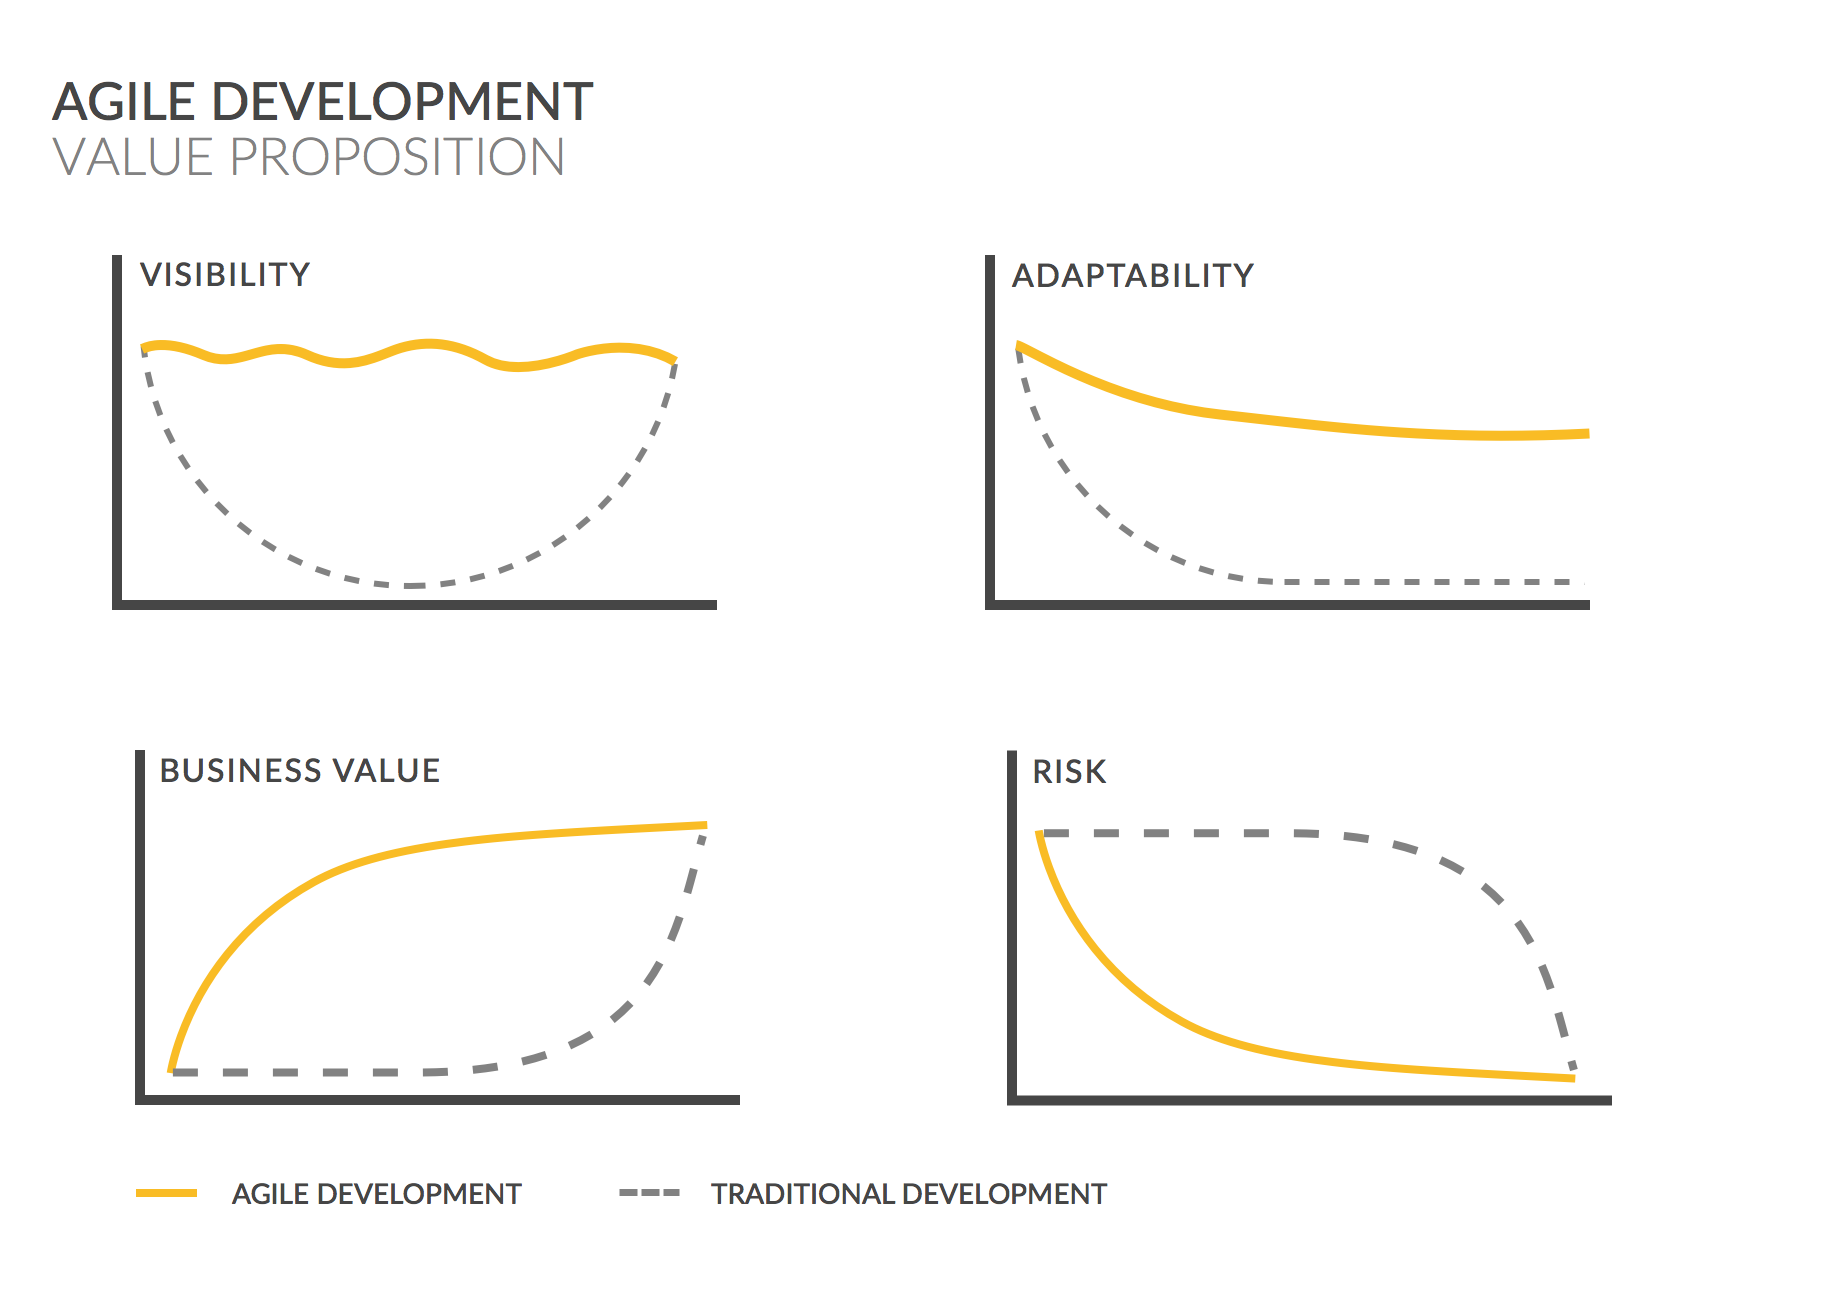
\includegraphics[scale=0.25]{images/travailBP1818/agile.png}
	\centering
	\caption{Comparaison méthodes agiles - traditionnelles}
	\label{agile}
\end{figure}

	Dans notre cas, nous utilisons la méthodologie \textit{Scrum}. Il s'agit de l'une des méthodes agiles les plus utilisée dont nous allons maintenant voir le détail.

\subsection{Déroulement des sprints}
\label{deroulementSprint}

	Scrum est une méthode de gestion de projet très répandue et prisée des adeptes de la philosophie Agile. Bien qu'elle soit plutôt simple à comprendre, elle reste néanmoins difficile à mettre en place et à maîtriser dans un projet. \\
	
	\subsubsection{Sprints}
	Nous avons vu plus haut que les méthodes Agiles préconisent de découper la réalisation du projet en un ensemble d'itérations courtes. Ici, ces dernières sont nommées \textbf{sprints} qui sont des périodes de deux semaines (ou parfois trois semaines lorsque des conditions particulières l'imposent comme une diminution des ressources à cause des vacances).
	
	\subsubsection{Le Product Backlog}
	Le product backlog est un référentiel contenant les exigences fonctionnelles et non foncitonnelles initiales définies par le client. Celui-ci est amené à évoluer à mesure que le projet avance.
	
	\subsubsection{User Story}
	Une user story, ou récit utilisateur, est la description d'une fonctionnalité métier à valeur business. Dans notre cas, il s'agit d'un fichier excel décrivant une fonctionnalité du point de vue utilisateur (\textit{En tant que..., je clique sur … dans le but de …}). Elle présente toutes les règles de gestions, prévoit tous les cas d'utilisation et contient aussi des maquettes afin que nous puissions construire l'IHM dans les meilleures conditions possibles.
	
	\subsubsection{Les rôles clés}
	Scrum définit différents rôles clés qui sont les suivants :
	\begin{itemize}
		\item Le \textbf{Product Owner} qui possède une vision globale sur le projet et dont l'objectif est de décrire et prioriser les élements du Product Backlog.
		\item Le \textbf{Scrum Master} dont l'objectif principal est s'assurer que la méthodologie Scrum est correctement appliquée et que ses valeurs sont intégrées par l'équipe.
		\item L'\textbf{équipe} qui se charge de réaliser le produit et donc ici le Fronting Digital
	\end{itemize}
	
	\subsubsection{Déroulement d'un sprint}
	Nos ressources se décomposent en une équipe fonctionnelle, de pilotage ainsi que de développement. Lors d'un sprint, l'équipe fonctionnelle collabore avec les métiers BP1818 et le product owner afin de pouvoir constituer un backlog suffisamment complet et ordonnancé pour plannifier le prochain sprint. Pour cela des \textbf{ateliers} sont régulièrement organisés entre ces deux parties afin de faire constamment évoluer le product backlog. Après cela, cette équipe est en charge de rédiger les \textbf{User Stories}. Une user story représente une exigence ou une fonctionnalité souhaitée par le client et décrit celle-ci de manière détaillée en précisant le comportement attendu, des maquettes pour l'IHM etc... : \textit{Lorsque je vais sur la page ... et que je clique sur le bouton ... l'action ... se déclenchera}. \\
	
	Une fois ces dernières validées, elles nous sont transmises, côté équipe de développement, afin que nous puissions les étudier. Dans un premier temps, l’ensemble de l’user story est découpée en tâches unitaires pouvant être réalisées par une unique ressource, qui seront consignées sous forme d’issue sous Github. Par la suite, une réunion de type \textbf{Sprint Planning} est organisée avec l'ensemble de l'équipe Sopra Steria dans l’optique de valider le contenu du sprint. Lors de ce sprint planning nous présentons l’ensemble des tâches découpées précédemment à l’équipe et exposons brièvement la manière dont nous les développerons afin que chacun puisse s’imprégner du travail qui sera réalisé et que les dernières modifications puissent être apportées. Ensuite, pour chacune des tâches ainsi dévoilées, une estimation de charge est réalisée via la méthode du \textbf{Poker Planning}. Il s’agit d’une pratique permettant d’estimer la complexité des fonctionnalités à développer en faisant interagir de manière ludique l’ensemble des parties prenantes. En effet, chaque participant possède des cartes indiquant différents niveaux de complexité (les niveaux représentent les nombres de la suite de Fibonacci). Lorsqu’une des tâches a été présentée par les développeurs, les participants choisissent la carte correspondant à leur estimation personnelle de la compléxité et la retourne tous en même temps. La discussion reprend tant qu’il n’y a pas l’unanimité sur la valeur de la complexité. Dans notre cas, un point de compléxité correspond à 0.75 jour de travail pour une ressource. Par exemple, si une tâche est validée à 5 points de complexité alors cette dernière devra être réalisée en 3.75 jours. Une fois les estimations terminées, certaines tâches sont choisies en fonction de leur priorité définie avec le product owner et du temps disponible pour le sprint et constituront le \textbf{Sprint Backlog}.\\
	
	A l'issue de cette réunion la phase de développement peut commencer. Elle inclut la conception détaillée des différentes tâches, le développement ainsi que les tests unitaires. Lorsque le développement est terminé le produit partiel est livré et part en phase de qualification. Cette phase est menée par l'équipe fonctionelle qui sera en charge d'effectuer toute une batterie de test afin de vérifier la conformité du produit à l'user story. Tous les bugs relevés sont consignés sous forme d'issue sur Github afin que nous puissions les corriger. Cette phase est en quelque sorte une phase de pré-recette nous permettant de nous affranchir d'un maximum d'anomalies avant de livrer l'application aux métiers.

\begin{figure}[h!]
	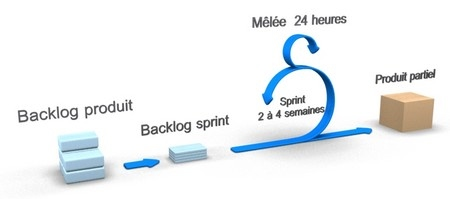
\includegraphics[scale=0.7]{images/travailBP1818/scrum.jpg}
	\centering
	\caption{Méthode Scrum}
	\label{scrum}
\end{figure}